\documentclass[a4paper, 12pt, final, garamond]{book}
\usepackage{cours-preambule}

\raggedbottom

\makeatletter
\renewcommand{\@chapapp}{\'Electrocin\'etique -- chapitre}
\makeatother

\begin{document}
\setcounter{chapter}{5}

\chapter{TD~: oscillateurs en RSF}

\section{Notation complexe}

Écrire, sous forme complexe, les équations différentielles suivantes~:
\[\tau \dv{u}{t} + u(t) = E_0\sin\wt
\qquad \qquad
\ddot{x} +  2\lambda \dot x + \w_0^2 x(t) =F_0\cos\wt\]

\section{Filtre de \textsc{Wien}}

\begin{minipage}{0.45\linewidth}
    On considère le circuit ci-contre avec $e(t) = E_m \cos(\wt)$. On note
    $u(t) = U_m \cos(\wt + \f)$ et on pose $H_m = U_m / E_m$ .
    \begin{enumerate}
        \item Déterminer les valeurs limites de $u(t)$ à basse et haute
            fréquences.
    \end{enumerate}
    Les courbes représentatives de $H_m (\w)$ et $\f(\w)$ sont
    fournies par les figures ci-dessous.
\end{minipage}
\hfill
\begin{minipage}{0.45\linewidth}
    \begin{center}
        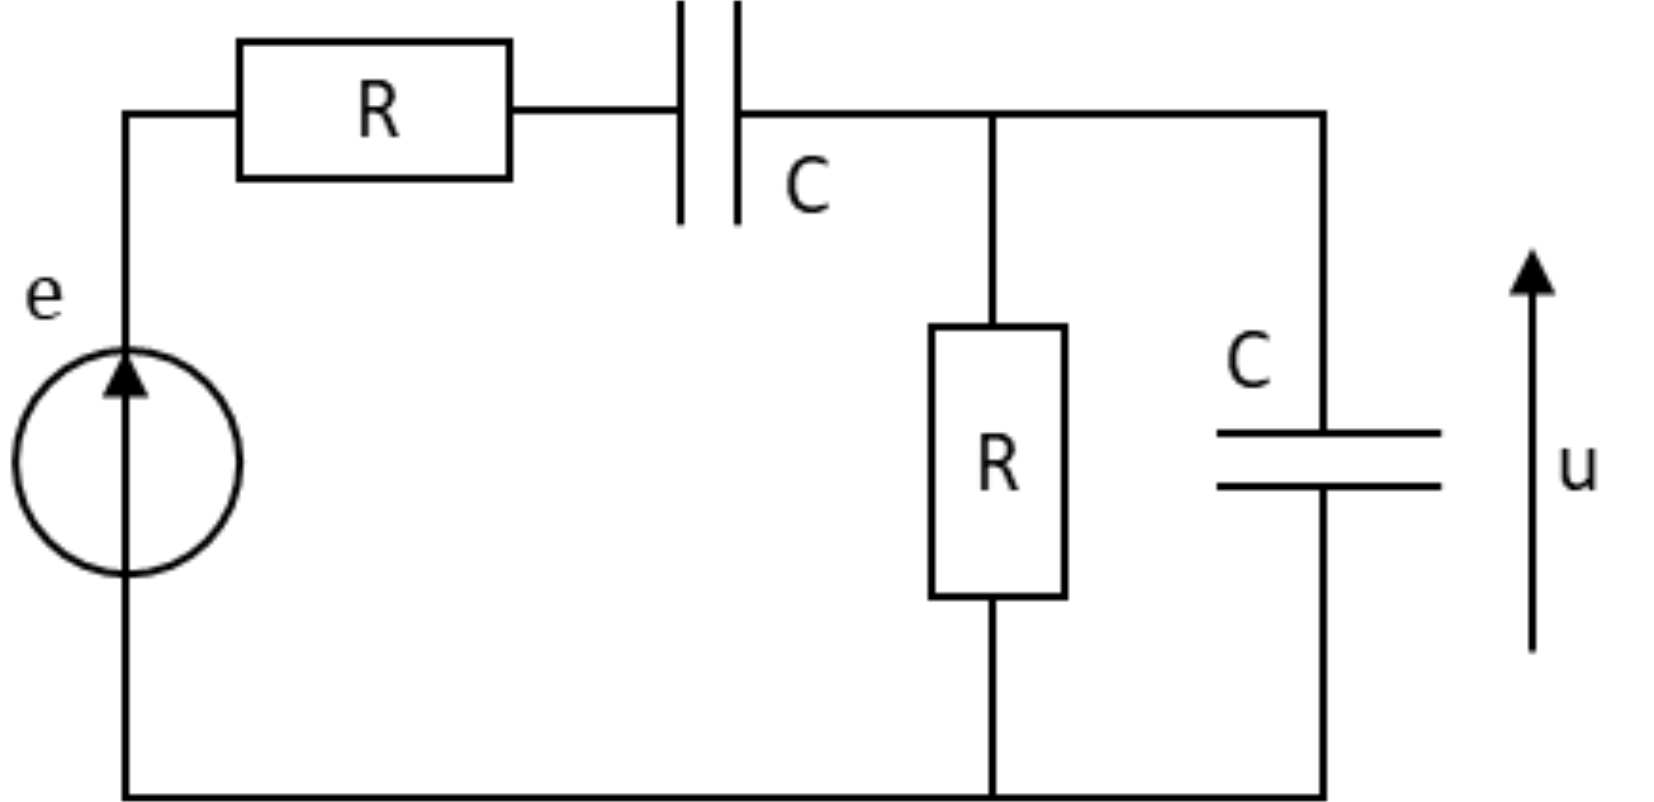
\includegraphics[width=\linewidth]{wien_1}
    \end{center}
\end{minipage}

\begin{minipage}{0.45\linewidth}
    \begin{center}
        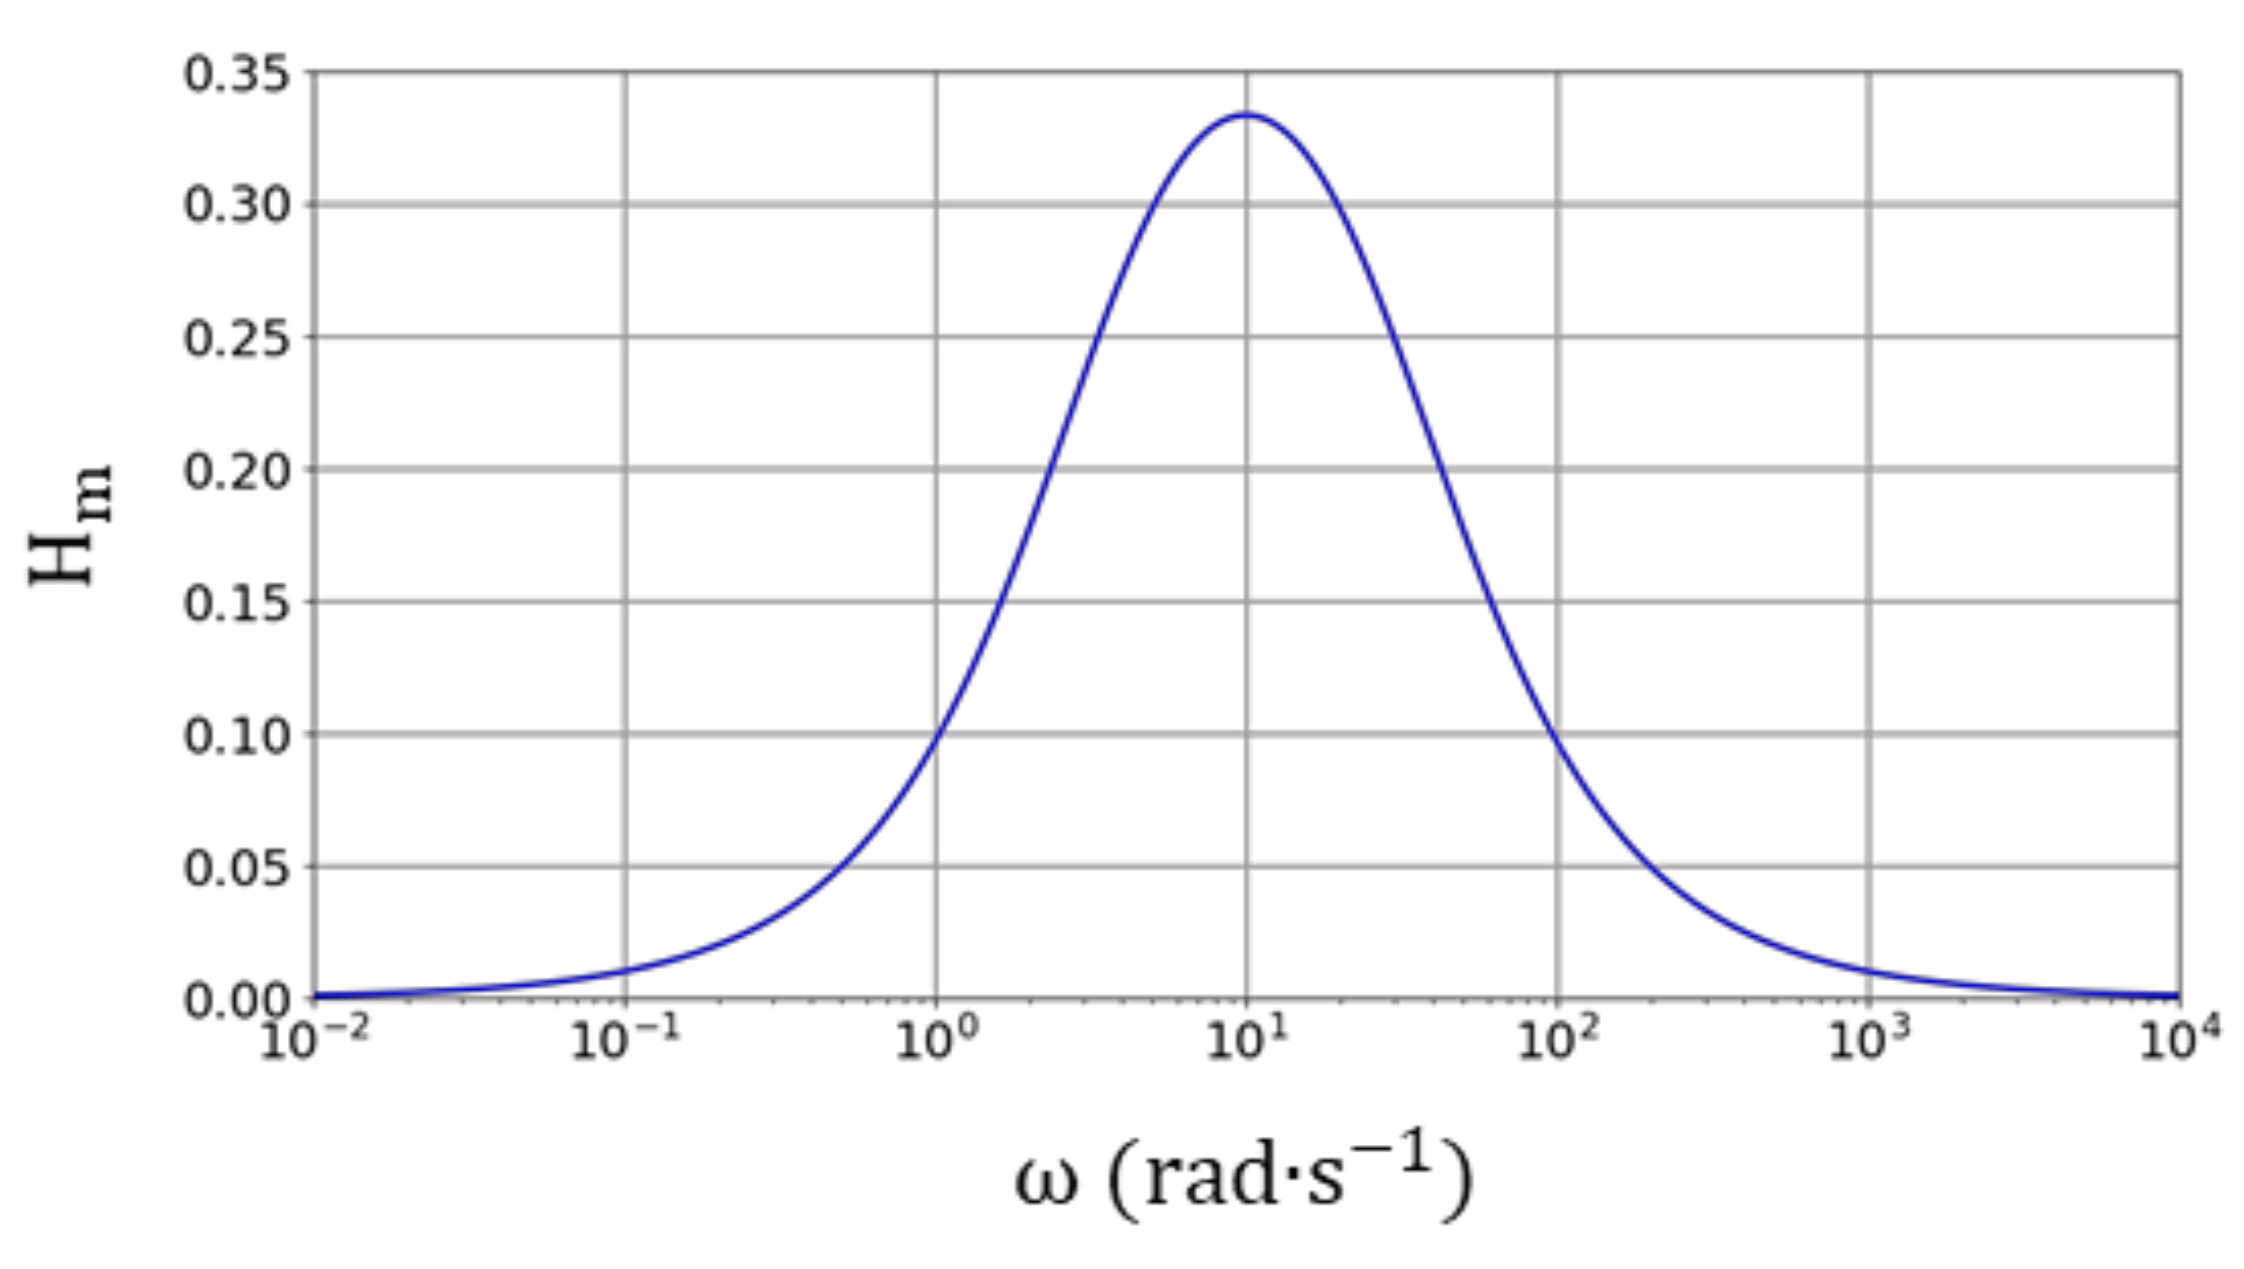
\includegraphics[width=\linewidth]{wien_3}
    \end{center}
\end{minipage}
\hfill
\begin{minipage}{0.45\linewidth}
    \begin{center}
        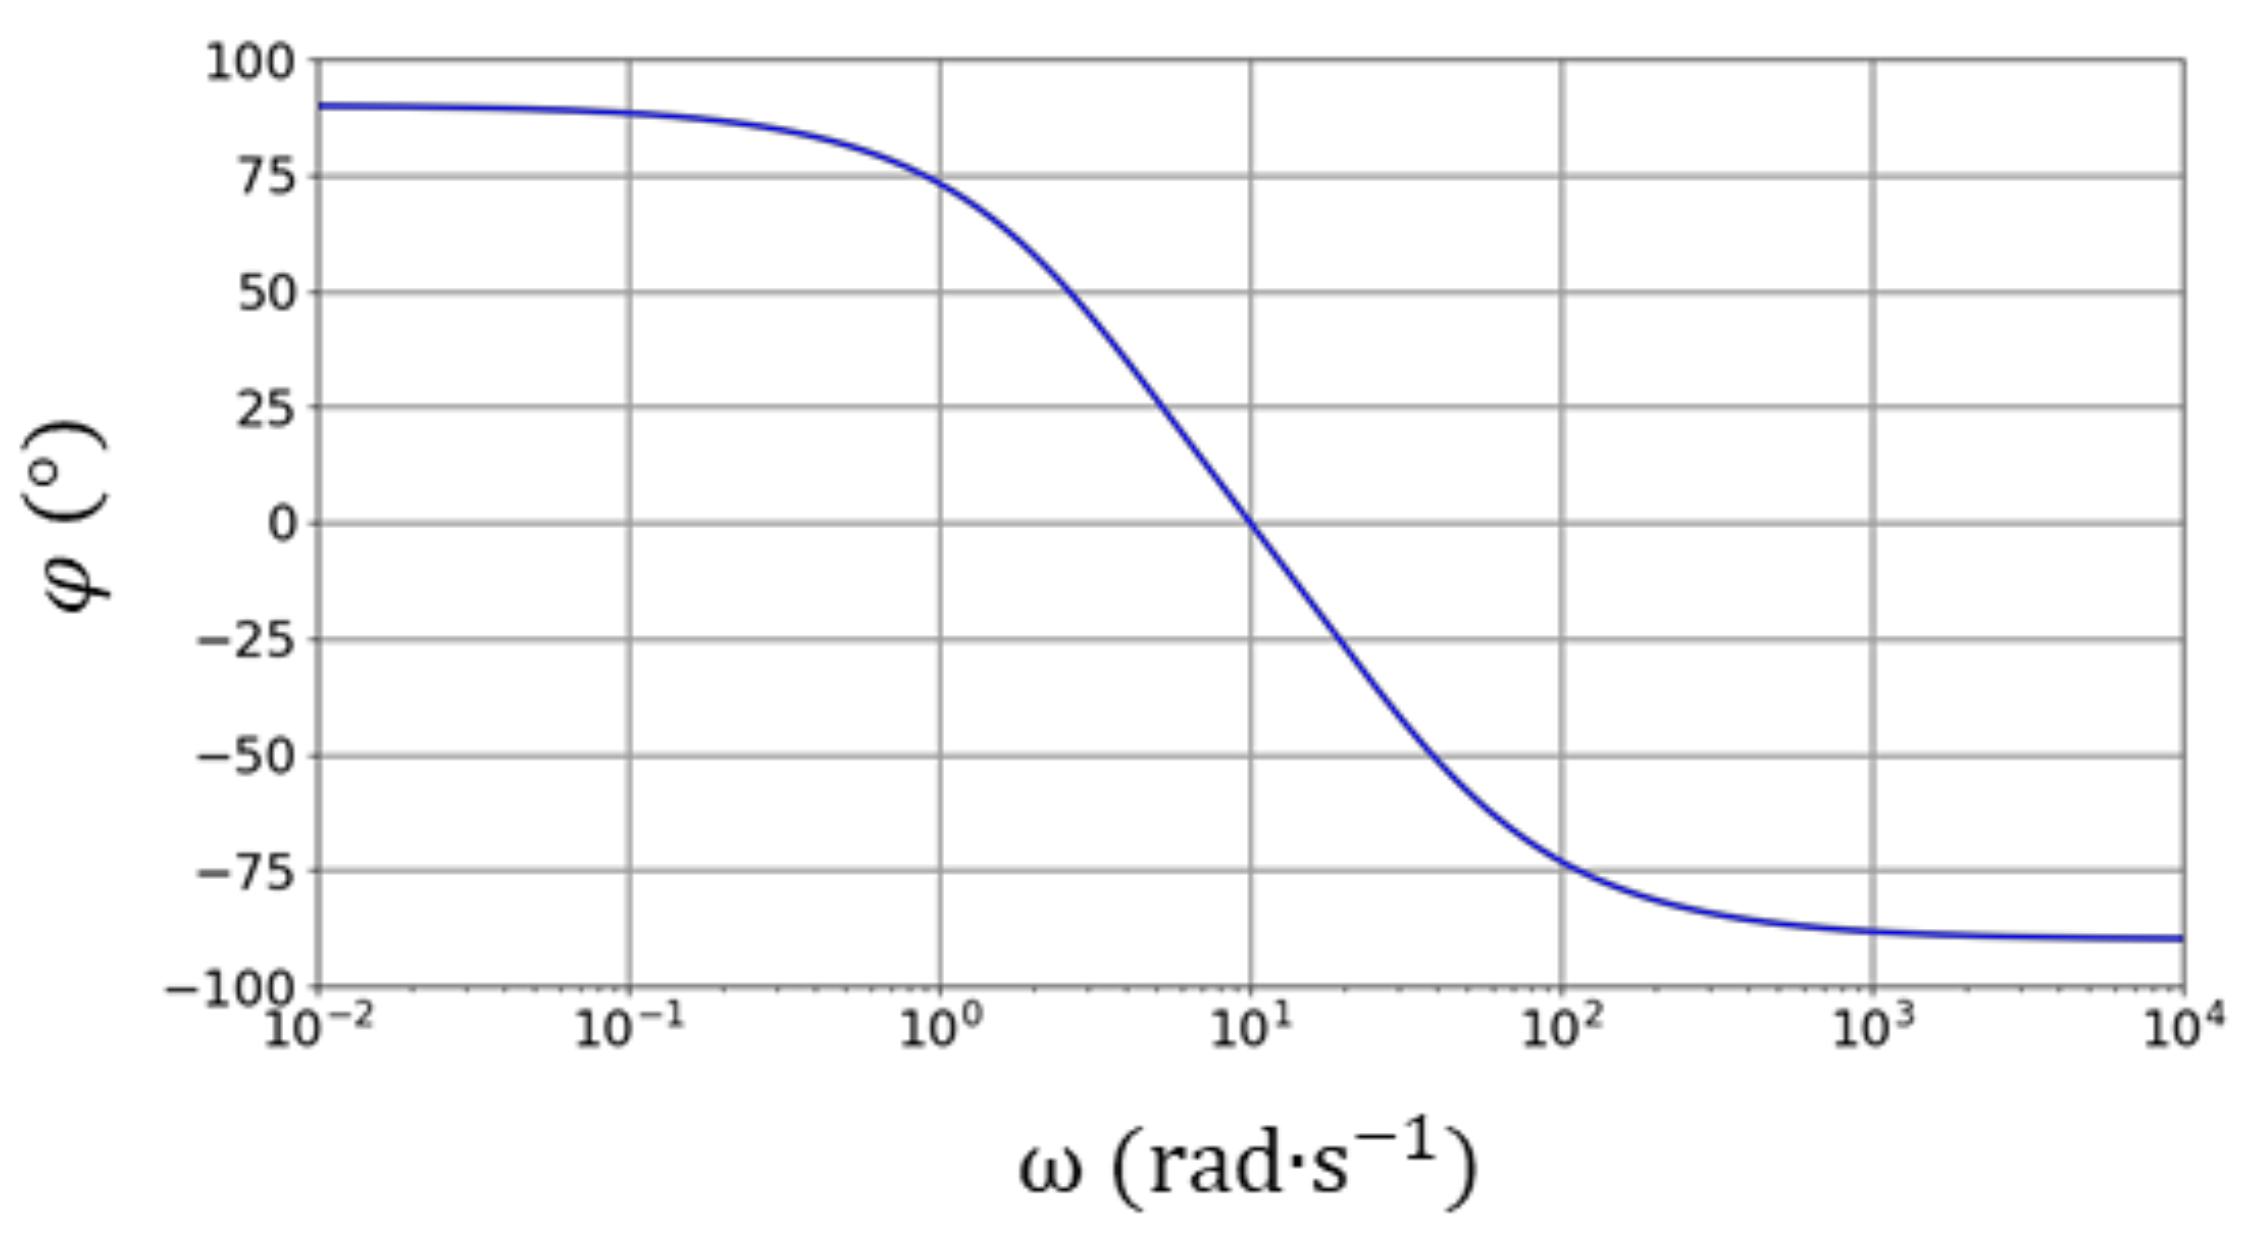
\includegraphics[width=\linewidth]{wien_2}
    \end{center}
\end{minipage}

\begin{enumerate}[start=2]
    \item Observe-t-on un phénomène de résonance en tension~? Justifier.
    \item Déterminer graphiquement la pulsation de résonance, les pulsations de
        coupure et la bande passante du filtre.
    \item Après avoir associé certaines impédances entre elles, établir
        l'expression de $\ul{H} = \ul{u} / \ul{e}$. La
        mettre sous la forme~:
        \[
            \ul{H}
                = \dfrac{H_0}{1 + \jj Q\left(x - \dfrac{1}{x}\right)}
            \qavec
            x = \dfrac{\w}{\w_0}
        \]
        avec $H_0$, $\w_0$ et $Q$ des constantes à exprimer en fonction
        (éventuellement) de $R$ et $C$.
    \item Déterminer graphiquement la valeur du produit $RC$.
\end{enumerate}

\section{Modélisation d'un haut-parleur}

\begin{minipage}{0.55\linewidth}
    On modélise la partie mécanique d'un haut-parleur comme une masse $m$, se
    déplaçant horizontalement le long d'un axe $(Ox)$. Cette masse est reliée
    à un ressort de longueur à vide $\ell_0$ et de raideur $k$ et subit une
    force de frottement fluide~: $\vec{f} = -\alpha \vec{v}$. Elle est par
    ailleurs soumise à une force $\vec{F}(t)$, imposée par le courant $i(t)$
    entrant dans le haut-parleur, qui vaut~: $\vec{F}(t) = K i(t) \vec{u}_x$
    où $K$ est une constante. On travaille dans le référentiel du laboratoire
    $(O, \vec{u}_x , \vec{u}_y)$. On suppose que le courant est de la forme
    $i(t) = I_m \cos(\wt)$.
\end{minipage}
\hfill
\begin{minipage}{0.45\linewidth}
    \begin{center}
        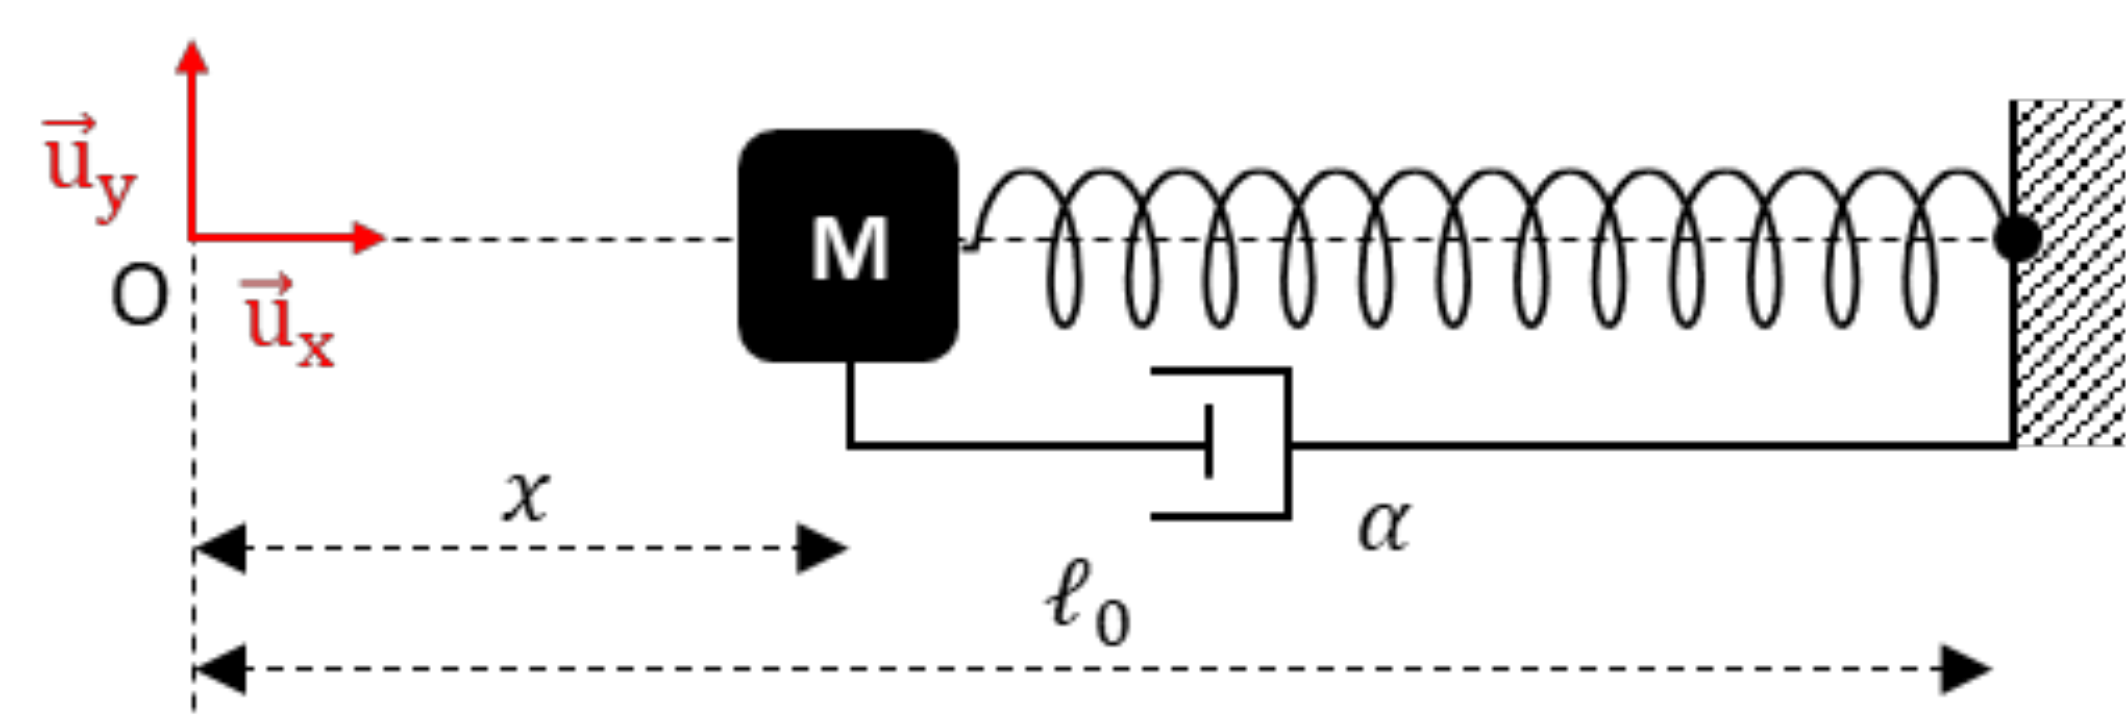
\includegraphics[width=.9\linewidth]{hp_1}
    \end{center}
\end{minipage}

\begin{rdefi}{Données}
    $m = \SI{10}{g}$, $K = \SI{200}{N.A^{-1}}$ et $I_m = \SI{1.0}{A}$.
\end{rdefi}

\begin{enumerate}
    \item Écrire l'équation différentielle vérifiée par $x(t)$, la position de
        la masse $m$.
    \item La mettre sous forme canonique et identifier les expressions de la
        pulsation propre $\w_0$ et du facteur de qualité $Q$.
    \item Justifier qu'en régime permanent: $x(t) = X_m \cos(\wt + \phi)$
    \item On pose $\ul{x}(t) = \ul{X}e^{\jwt}$. Déterminer
        l'expression de l'amplitude complexe $\ul{X}$.
    \item Exprimer $X_m(\w)$. Existe-t-il toujours une résonance?
\end{enumerate}

On a tracé ci-dessous les courbes de $X_m (\w)$ et de
$\phi(\w)$. L'axe des abscisses est en échelle logarithmique.

\begin{center}
    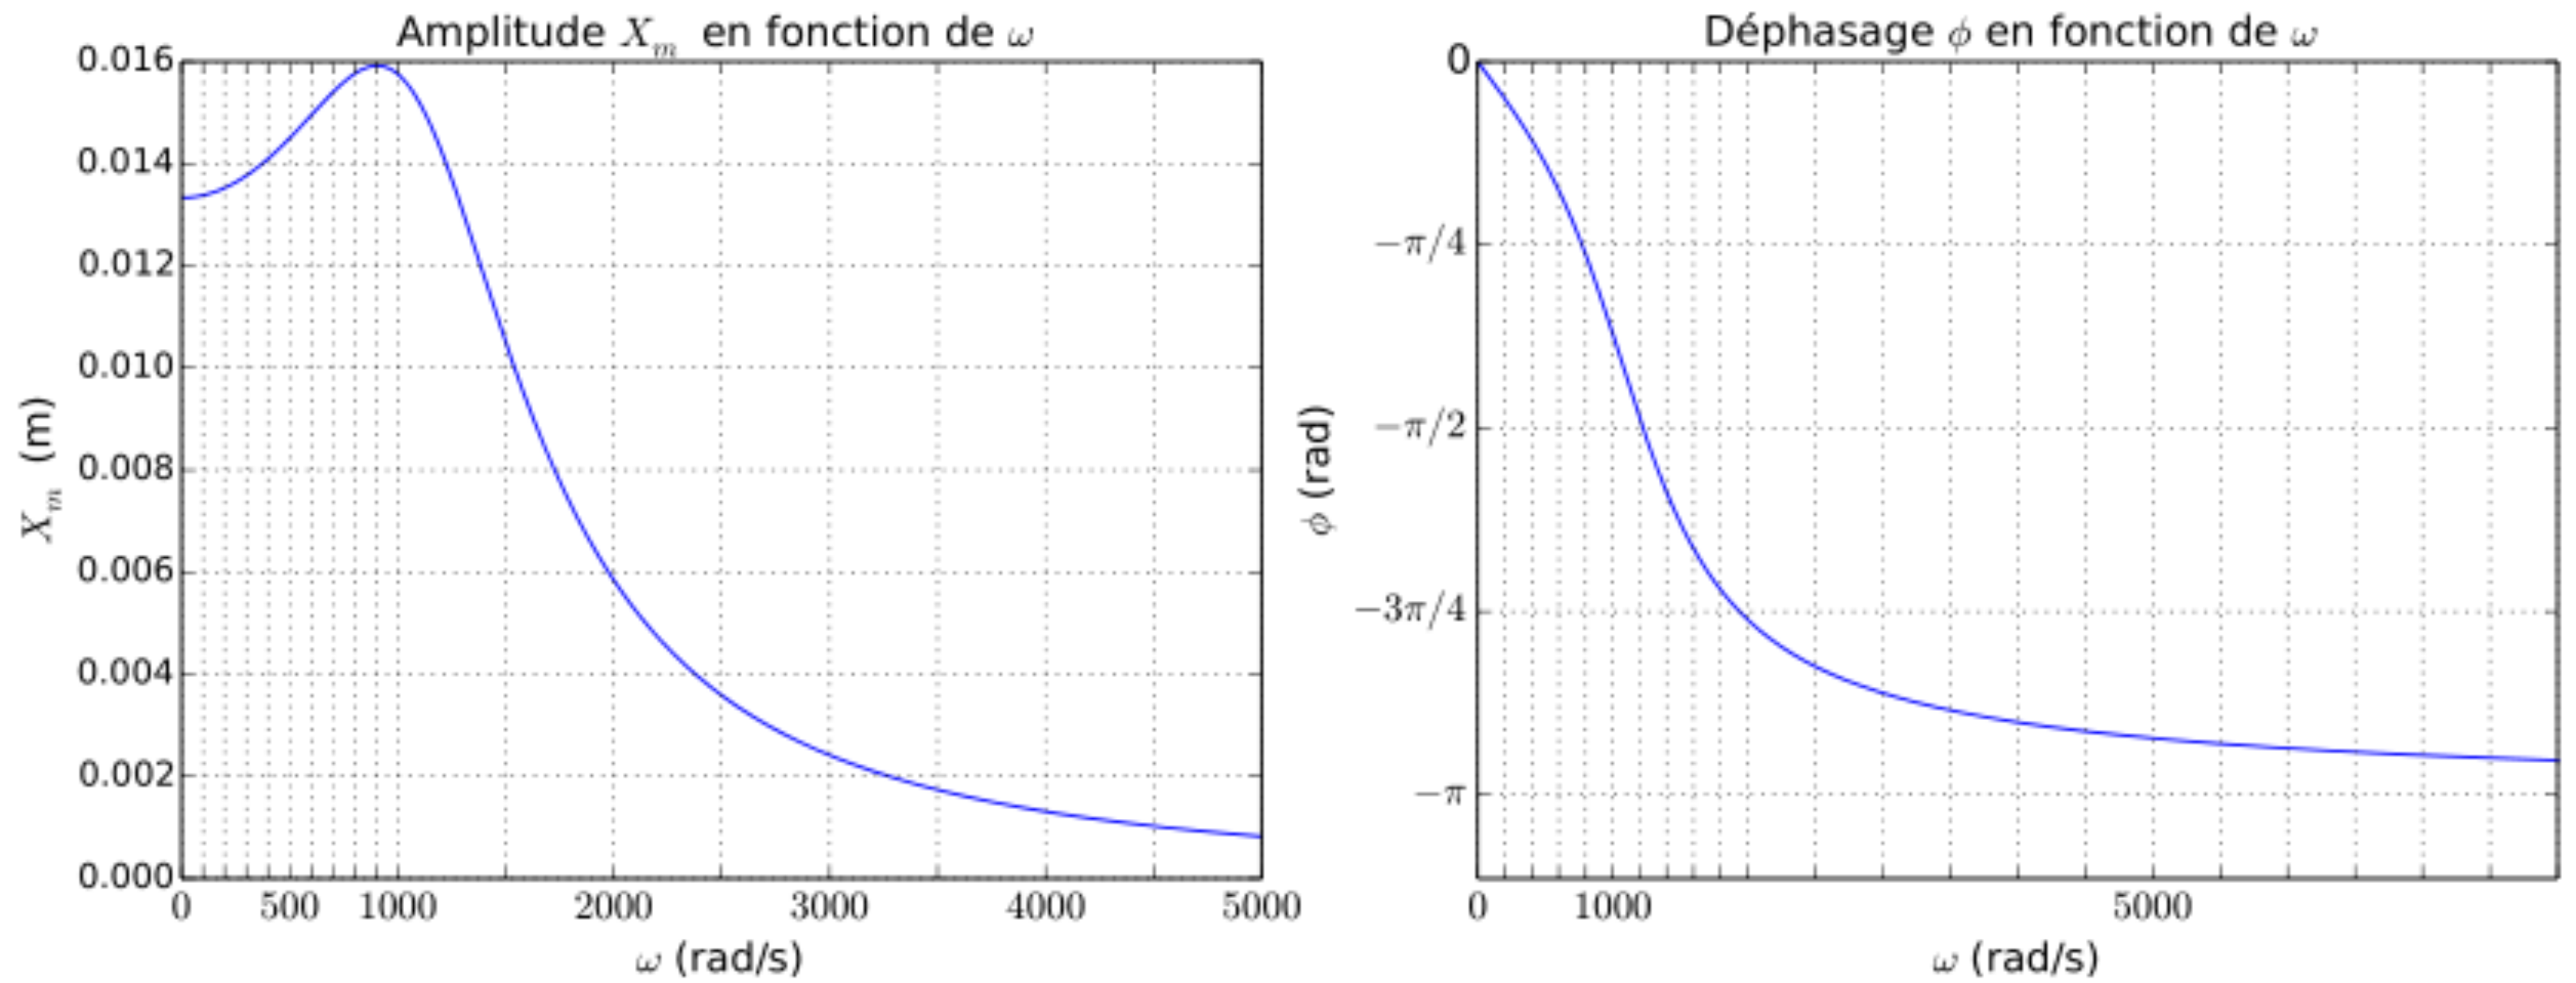
\includegraphics[width=.8\linewidth]{hp_2}
\end{center}

\begin{enumerate}[start=6]
    \item Pour quelle pulsation le déplacement est-il en quadrature de phase
        avec la force excitatrice~? Déterminer alors graphiquement la pulsation
        propre $\w_0$.
\end{enumerate}

\section{Résonance d'un circuit bouchon}

\begin{minipage}{0.55\linewidth}
    
On considère le circuit $RLC$ représenté ci-contre, composé d'un
résistor, de résistance $R$, d'une bobine idéale d'inductance $L$,
d'un condensateur idéal, de capacité $C$, alimenté par une source
idéale de tension, de f.e.m. $e(t)=E_0\cos(\wt)$. On se place en
régime sinusoïdal forcé.
\end{minipage}
\hfill
\begin{minipage}{0.45\linewidth}
    \begin{center}
        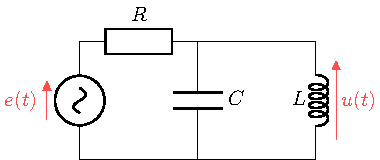
\includegraphics[width=\linewidth]{bouchon_plain}
    \end{center}
\end{minipage}

\begin{enumerate}
    \item Exprimer l'amplitude complexe $\ul{U}$ de $u(t)$ en
        fonction de $E_0$, $R$, $L$, $C$ et $\w$.
    \item Établir qu'il existe un phénomène de résonance pour la tension
        $u(t)$. Préciser la pulsation $\w_0$ à laquelle ce phénomène se
        produit et la valeur de l'amplitude réelle de $u(t)$ à cette
        pulsation.
    \item Mettre l'amplitude réelle $U$ de $u(t)$ sous la forme: \[U =
            \dfrac{E_0}{\sqrt{1 + Q^2\left(\dfrac{\w}{\w_0} -
        \dfrac{\w_0}{\w}\right)^2}}\] avec $Q$ un facteur sans
        dimension à exprimer en fonction de $R,L$ et $C$.
    \item Exprimer la bande passante $\Delta\w$ de cette résonance en
        fonction de $Q$ et $\w_0$.
    \item En déduire les valeurs numériques de $C$ et $E_0$ à l'aide du
        graphe ci-dessous représentant l'amplitude réelle de $u(t)$ en
        fonction de la fréquence $f=\w/2\pi$, sachant que $L= \SI{1}{mH}$ et
        $R= \SI{1}{k\Omega}$.
\end{enumerate}

\begin{center}
    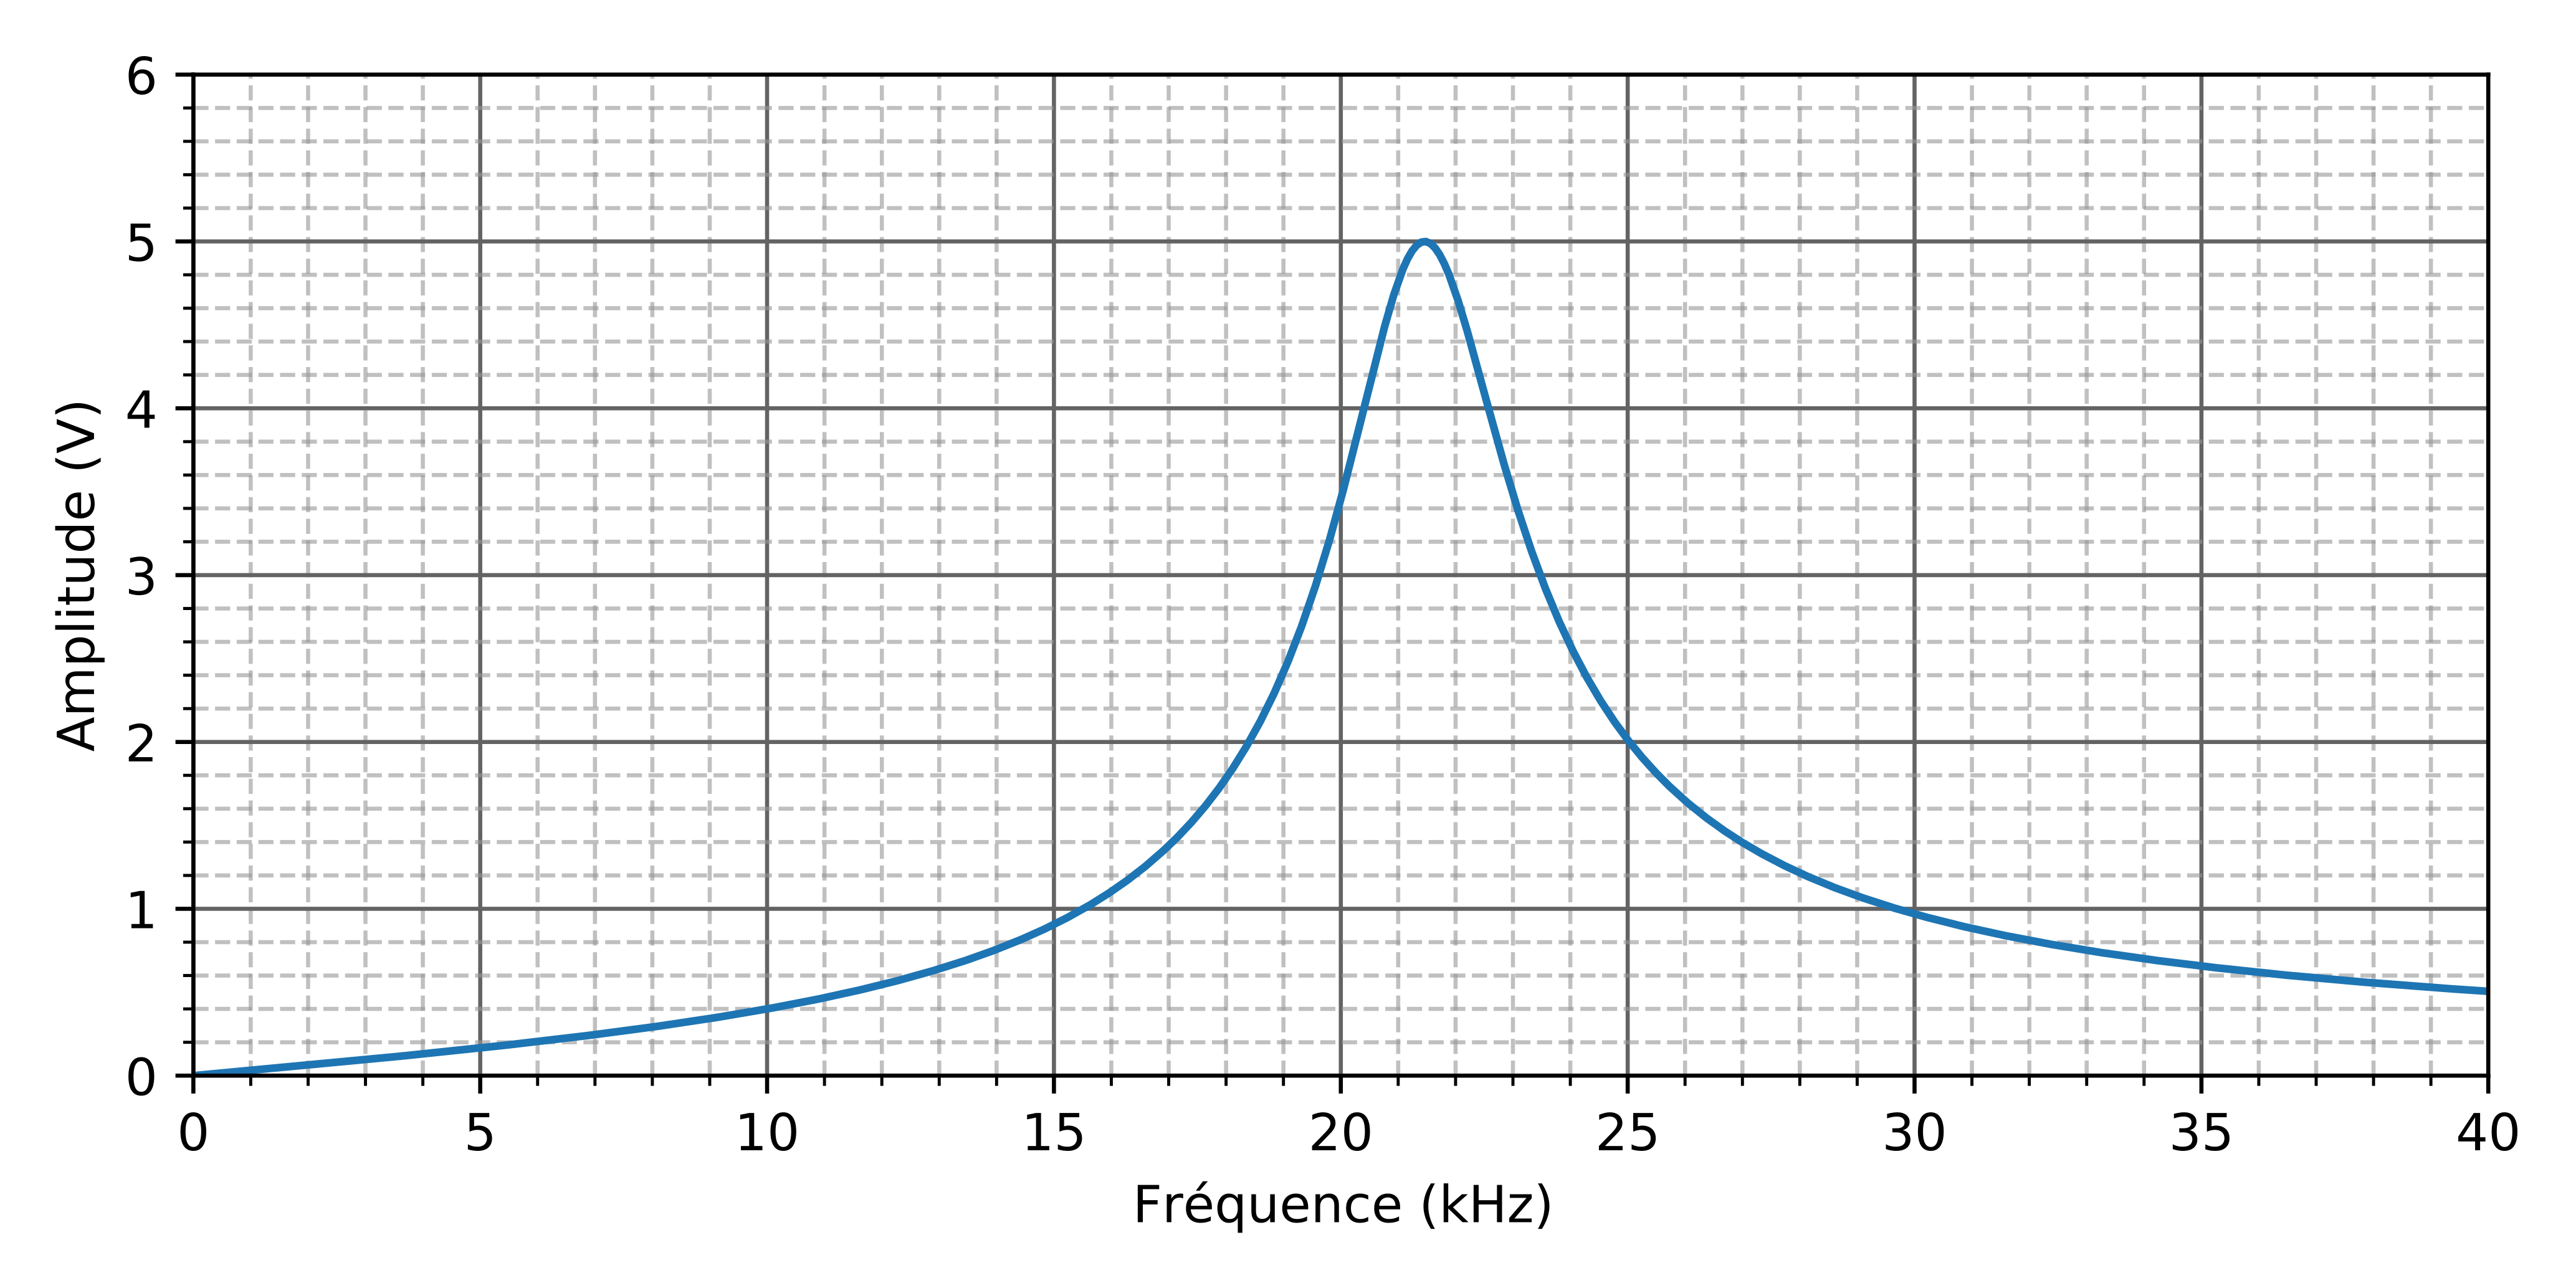
\includegraphics[width=.8\linewidth]{bouchon_2}
\end{center}

\section{Système à deux ressorts}
\begin{minipage}{0.60\linewidth}
    Un point matériel $M$, de masse $m$, peut se déplacer sur une tige
    \emph{horizontale} parallèle à l'axe $Ox$ au sein d'un fluide visqueux qui
    exerce sur lui la force de frottement $\vec{f} = - h\vec{v}$ avec
    $\vec{v}$ le vecteur vitesse de $M$ dans le référentiel galiléen
    $\mathcal{R}$ du laboratoire. Les frottements entre $M$ et l'axe
    horizontal sont négligeables. On repère $M$ par son abscisse $x(t)$.
\end{minipage}
\hfill
\begin{minipage}{0.35\linewidth}
    \begin{center}
        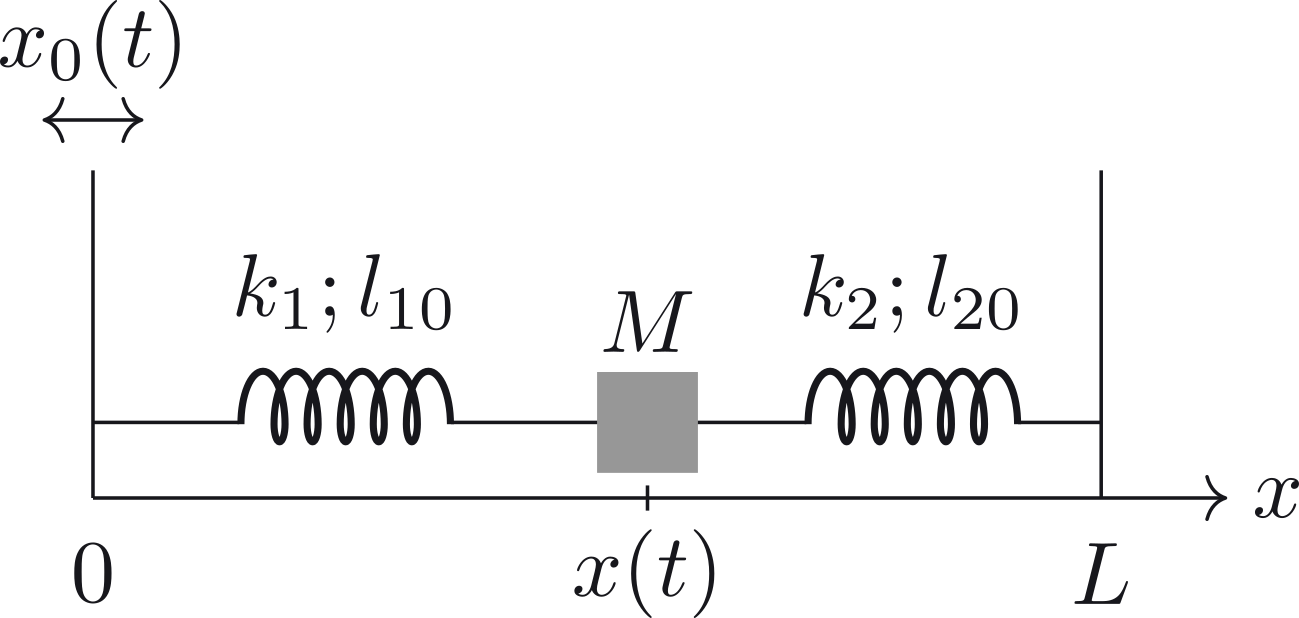
\includegraphics[width=\linewidth]{ressort-double_1}
    \end{center}
\end{minipage}

$M$ est relié à deux parois verticales par deux ressorts de raideurs $k_1$
et $k_2$, de longueurs à vide $\ell_{10}$ et $\ell_{20}$. Celle de droite est
immobile en $x = L$, celle de gauche, d'abscisse $x_0 (t)$, est animée d'un
mouvement d'équation horaire $x_0 (t) = X_{0m} \cos(\wt)$. On supposera
que $L = \ell_{10} + \ell_{20}$.

\begin{enumerate}
    \item Identifier les différentes forces s'exerçant sur $M$.
    \item Déterminer la position d'équilibre $x_{\eq}$ de $M$ lorsque la paroi
        de gauche est immobile en $x = 0$.
    \item On introduit $X = x - x_{\eq}$. Établir l'équation différentielle
        vérifiée par $X$ lorsque la paroi bouge.
\end{enumerate}
    Pour étudier le régime sinusoïdal forcé, on introduit les grandeurs
    complexes $\ul{x}_0(t) = X_{0m} \exp(\jj\wt)$, $X(t) = X_m \exp(\jj(\wt +
    \f))$ et $v(t) = V_m \exp(\jj(\wt + \phi))$ associées à $x_0(t)$, $X(t)$ et
    $v(t) = \dot X(t)$.
\begin{enumerate}[resume]
    \item Définir les amplitudes complexes $\ul{X}_0$, $\ul{X}$ et $\ul{V}$ de
        $x_0(t)$, $X(t)$ et $v(t)$.
    \item En exprimant $\w_0$, $Q$ et $\alpha$ en fonction des données du
        problème, établir la relation~: \[\ul{V} = \dfrac{\alpha}{1 +
        \jj Q\left(\dfrac{\w}{\w_0} - \dfrac{\w_0}{\w}\right)} \ul{X}_0\]
    \item Mettre en évidence l'existence d'une résonance de vitesse.
\end{enumerate}

\section{Résonance d'intensité dans un circuit RLC parallèle}

\begin{minipage}{0.60\linewidth}
    L'antenne d'un émetteur radio peut être modélisée par un circuit électrique
    équivalent composé de l'association en parallèle d'une résistance $R$,
    d'une bobine d'inductance $L$ et d'un condensateur de capacité $C$.
    \smallbreak
    L'antenne est alimentée par une source idéale de courant dont l'intensité
    caractéristique varie de manière sinusoïdale dans le temps: $i(t) = I_0
    \cos(\wt)$.
\end{minipage}
\hfill
\begin{minipage}{0.35\linewidth}
    \begin{center}
        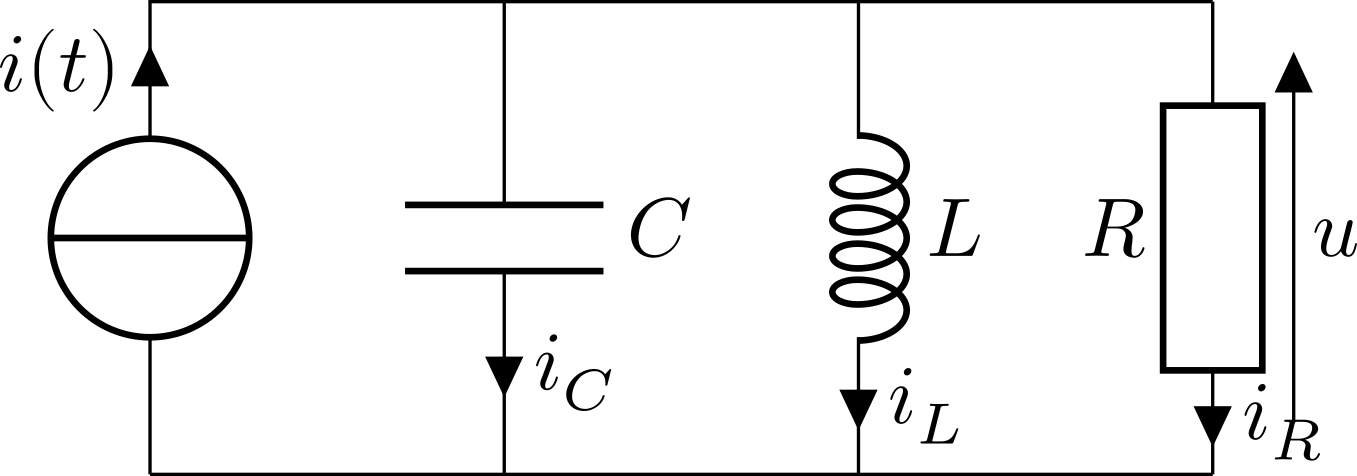
\includegraphics[width=\linewidth]{rlc_parr}
    \end{center}
\end{minipage}

On s'intéresse à la manière dont l'amplitude de la tension $u(t)$ aux
bornes de l'antenne, qui correspond au signal envoyé, dépend de
$\w$.

\begin{enumerate}
    \item Déterminer l'impédance complexe de l'association des dipôles $R,L$ et
        $C$.
    \item En déduire l'amplitude complexe $\ul{U}$ de la tension $u$ en fonction
        de $\w$, $I_0$, $R$, $L$ et $C$.
    \item Pour quelle pulsation l'amplitude réelle $U$ de $u$ prend-elle sa
        valeur maximale notée $U_\text{max}$~? Conclure sur la fréquence à
        utiliser.
    \item Représenter le graphe donnant $U$ en fonction de la pulsation réduite
        $x=\w/\w_0$ avec $\w_0=1/\sqrt{LC}$.
    \item Exprimer la largeur de la bande passante $\Delta\w$.
    \item On se place dans le cas $R = \SI{7}{\Omega}$, $L = \SI{1.2e-8}{H}$ et $C =
        \SI{2.3e-10}{F}$. Calculer la valeur de l'acuité $A_c = \w_0/\Delta\w$
        de la résonance. Interpréter sa dépendance en $R$.
\end{enumerate}

\section{Condition de résonance}
\begin{minipage}{0.60\linewidth}
    Le circuit ci-contre est alimenté par une source de tension sinusoïdale de
    f.é.m. $e(t) = E_0 \cos( \wt)$. On s'intéresse à la tension $u(t)$
    aux bornes du résistor et de la capacité montés en parallèle.

    On pose~: $\w_0 =\dfrac{1}{\sqrt{LC}}$, $\xi =
    \dfrac{R}{2}\sqrt{\dfrac{C}{L}}$ et $x = \dfrac{\w}{\w_0}$.
\end{minipage}
\hfill
\begin{minipage}{0.35\linewidth}
    \begin{center}
        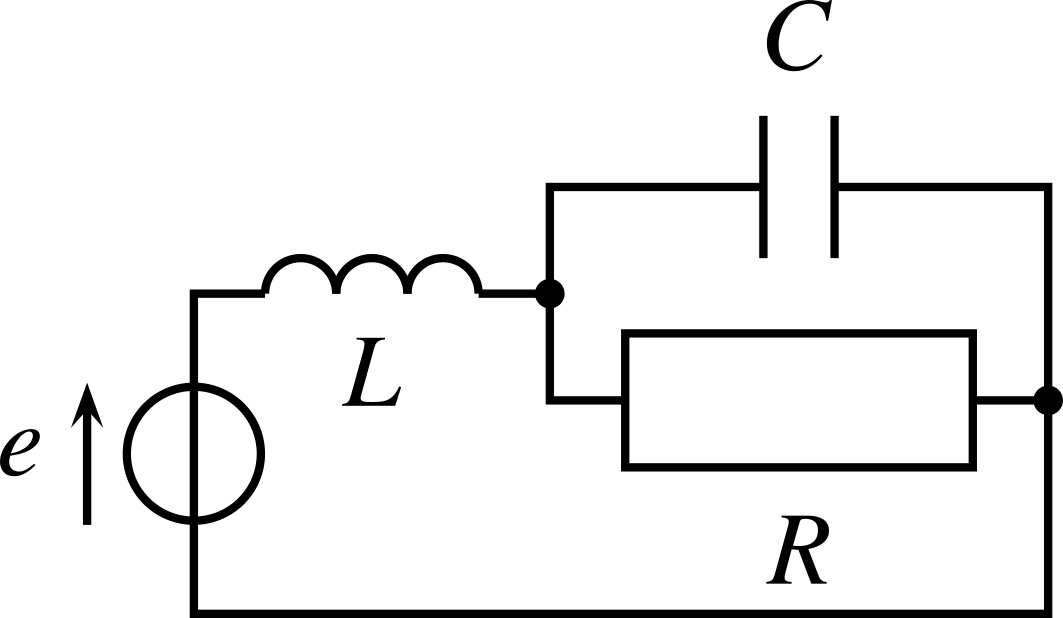
\includegraphics[width=\linewidth]{cond_res}
    \end{center}
\end{minipage}

\begin{enumerate}
    \item Établir l'expression du signal complexe $\ul{u}$ associé à
        $u(t)$ en régime sinusoïdal forcé, en fonction de $E_0$, $x$ et
        $\xi$.
    \item Étudier l'existence éventuelle d'une résonance pour la tension
        $u(t)$.
\end{enumerate}

\end{document}
